\documentclass[14pt]{beamer}
\usepackage[T2A]{fontenc}
\usepackage[utf8]{inputenc}
\usepackage[english,russian]{babel}
\usepackage{amssymb,amsfonts,amsmath,mathtext}
\usepackage{cite,enumerate,float,indentfirst}
\usepackage{longtable}  
\graphicspath{{../assets/}{images/}} 

\usetheme{Pittsburgh}
\usecolortheme{whale}

\setbeamercolor{footline}{fg=blue}
\setbeamertemplate{footline}{
  \leavevmode%
  \hbox{%
  \begin{beamercolorbox}[wd=.333333\paperwidth,ht=2.25ex,dp=1ex,center]{}%
    А. С. Тощев, К(П)ФУ
  \end{beamercolorbox}%
  \begin{beamercolorbox}[wd=.333333\paperwidth,ht=2.25ex,dp=1ex,center]{}%
    Казань, 2017
  \end{beamercolorbox}%
  \begin{beamercolorbox}[wd=.333333\paperwidth,ht=2.25ex,dp=1ex,right]{}%
  Стр. \insertframenumber{} из \inserttotalframenumber \hspace*{2ex}
  \end{beamercolorbox}}%
  \vskip0pt%
}

\newcommand{\itemi}{\item[\checkmark]}

\title{\small{Диссертация на соискания ученой степени кандидата технических наук по специальности 05.13.11}}
\author{
Интеллектуальная система повышения эффективности IT службы предприятия\\
\small{%
\emph{Соискатель:} А.C. Тощев\\%
\emph{Руководитель:} проф., д.ф.-м.н. А.М.Елизаров}\\%
\vspace{30pt}%
Казанский (Приволжский)\\
федеральный университет%
\vspace{20pt}%
}
\date{\small{Казань, 2017}}

\begin{document}

\maketitle


\begin{frame}
\frametitle{Термины и обозначения}
\begin{enumerate}
    \item ITIL~-- общепринятая методология в области поддержки IT;
    \item Инцидент~-- проблема, возникшая в результате работы ПО и приведшая к полной или частичной невозможности работы;
    \item TSS1~-- системный администратор 3 категории;
    \item TU~-- интеллектуальная система повышения эффективности ИТ-службы предприятия.
  
\end{enumerate}
\end{frame}


  \begin{frame}
   \frametitle{Содержание доклада}
    \tableofcontents
   \end{frame}


\AtBeginSection[] % Do nothing for \subsection*
{
\begin{frame}
\frametitle{}
\tableofcontents[current]
	
\end{frame}
}
% 
%    INTRODUCTION
%
\section[Введение]{Введение}

\begin{frame}
\frametitle{Цели и задачи}
\begin{itemize}
  \item \textbf{Предмет исследования} процесс регистрации и устранения проблемных ситуаций, возникающих в IT-инфраструктуре предприятия;
  \item \textbf{Цель исследования} разработка интеллектуальной системы повышения эффективности деятельности IT-службы предприятия;
  \item \textbf{Актуальность} определяется потребностью предприятий IT-отрасли в интеллектуальных системах, повышающих эффективность служб, поддерживающих IT-инфраструктуру этих предприятий.
\end{itemize}
\end{frame}

\begin{frame}
\frametitle{Близкие исследования}
\begin{enumerate}
 \item Институт Чиная (Индия) - Е. Джубилсон и П. Дханавантини;
 \item Институт Ганновера (Германия) – Р. Брунс и Дж. Данкель;
 \item СПбГУ (Россия) - В.И. Золотарев;
 \item Сингапур – С. Фу и П. Леонг;
 \item IBM Watson (IBM) - А. Гоэль;
 \item GATE3 (Университет Шеффилда (Великобритания)) – Г. Каллаган;
 \item OpenCog (США) –  Б. Герцель;
 \item NARS (Китай) – П. Вонг.
\end{enumerate}
\end{frame}



\begin{frame}
\frametitle{Обзор существующих решений}
\begin{table}
	
\small
\begin{tabular} {|p{5cm}|p{1cm}|p{1.5cm}|p{1.5cm}|}

\hline
\textbf{Критерий сравнения} & HP Open View & Service NOW & IBM Watson\\
\hline
   Мониторинг & Да & Да & Да  \\
   \hline
   Регистрация инцидентов & Да & Да & Да \\
   \hline
   Управление системами & Да & Нет & Нет  \\
   \hline 
   Создание цепи обработки & Да & Да & Нет \\
   \hline 
   Запросы на естественном языке & Нет & Нет & Да \\
   \hline 
   Поиск решений & Нет & Нет & Да \\
   \hline 
   Применение решений & Нет & Нет & Нет  \\
   \hline
   Обучение & Нет & Нет & Нет \\
   \hline
   Логические рассуждения & Нет & Нет & Нет  \\
   \hline
  
\end{tabular}
\end{table}
\end{frame}

\begin{frame}
\frametitle{Методы исследования}
\begin{enumerate}
  \item \textbf{Теоретические методы}
  \begin{itemize}
    \item Имитационное моделирование;
    \item Теория баз знаний в области искусственного интеллекта.
  \end{itemize}
   \item \textbf{Специальные методы}
  \begin{itemize}
    \item Экспериментальное моделирование;
    \item Cистемное моделирование.
  \end{itemize}
  
   \item \textbf{Экспериментальные методы}
  \begin{itemize}
    \item Метод наблюдений;
    \item Метод проведения экспериментов.
  \end{itemize}

\end{enumerate}
\end{frame}


\begin{frame}
\frametitle{Соответствие паспорту специальности}

\begin{table}
	
\small

\begin{tabular} {|p{5cm}|p{5cm}|}


 \hline
\textbf{Направление исследования} & Результат работы\\

\hline
   Языки программирования и системы программирования, семантика программ & Разработана семантическая модель организации хранения знаний \\
   \hline
  Системы управления базами данных и знаний & Разработан прототип Thinking Understanding (TU) системы хранения знаний и принятия решений в сфере поддержки ИТ-инфраструктуры предприятия, который был испытан на модельных данных\\
   \hline
    \end{tabular}
\end{table}
\end{frame}

\begin{frame}
\frametitle{Соответствие паспорту специальности}

\begin{table}
	
\small

\begin{tabular} {|p{5cm}|p{5cm}|}


 \hline
\textbf{Направление исследования} & Результат работы\\

 \hline
   Модели и методы создания программ и программных систем для параллельной и распределенной обработки данных, языки и инструментальные средства параллельного программирования & Разработан метод параллельной обработки экспертной информации c возможностью обучения при помощи прототипа TU \\
   \hline
 \end{tabular}
\end{table}
\end{frame}

\begin{frame}
\frametitle{Список публикаций}
 Основные результаты по теме диссертации изложены в 10 печатных изданиях:
\begin{itemize}
	\item Scopus:2;
	\item Web of science:1;
	\item РИНЦ:4;
	\item Перечень ВАК: 2;
	\item ACM: 2.
\end{itemize}
\end{frame}

\begin{frame}
\frametitle{Список публикаций}

\begin{itemize}
	\item Тощев, А.С. К новой концепции автоматизации программного обеспечения [Текст] / А. С. Тощев // Труды Математического центра имени Н.И. Лобачевского. «Лобачевские чтения — 2011. Казань, 31 октября – 4 ноября 2011». –– 2011. –– Т. 44, No 4. –– С. 279 – 282; 
	\item Toshchev, A. Thinking-Understanding approach in IT maintenance domain automation [Text] / A. Toshchev, M. Talanov, A. Krehov // Global Journal on Technology: 3rd World Conference on Information Technology (WCIT-2012). — 2013. — Vol. 3. — P. 879 – 894;
	
\end{itemize}
\end{frame}

\begin{frame}
\frametitle{Список публикаций}

\begin{itemize}
	\item Тощев, А.С. Архитектура и реализация интеллектуального агента для автоматической обработки входящих заявок с помощью искусственного интеллекта и семантических сетей [Текст] / А.С. Тощев, М.О. Таланов // Ученые записки Института социально-гуманитарных знаний. –– 2014. –– Т. 2. –– С. 288 – 292; 
	\item Toshchev, A. Computational emotional thinking and virtual neurotransmitters [Text] / A. Toshchev, M. Talanov // International Journal of Synthetic Emotions (IJSE). — 2014. — Vol. 5. — P. 30 – 35;
	
\end{itemize}
\end{frame}


\begin{frame}
\frametitle{Список публикаций}

\begin{itemize}
	\item Toshchev, A. Appraisal, coping and high level emotions aspects of computational emotional thinking [Text] / A. Toshchev, M. Talanov // International Journal of Synthetic Emotions (IJSE). — 2015. — Vol. 6. — P. 65 – 72; 
	\item Toshchev, A. Thinking model and machine understanding in automated user request processing [Text] / A. Toshchev // CEUR Workshop Proceedings. — 2014. — Vol. 1297. — P. 224 – 226;
\end{itemize}
\end{frame}


\begin{frame}
\frametitle{Список публикаций}

\begin{itemize}
	\item Тощев, А.С. Возможности автоматизации разрешения инцидентов для области удаленной поддержки информационной инфраструктуры предприятия [Текст] / А.С. Тощев // Экономика и менеджмент систем управления. –– 2015. –– Т. 4. –– С. 293 – 295;
	\item Toshchev, A. Thinking lifecycle as an implementation of machine understanding in software maintenance automation domain [Text] / A. Toshchev, M. Talanov // 9th KES International Conference, KES-AMSTA. -- 2015. — Vol. 38. -- P. 301 – 310;
\end{itemize}
\end{frame}

\begin{frame}
\frametitle{Список публикаций}

\begin{itemize}
	\item Тощев, А.C. Вычислительная модель эмоций в интеллектуальных информационных системах [Текст] / А.C. Тощев, М.О. Таланов // Электронные библиотеки. –– 2015. –– Т. 18. –– С. 225 – 235;
	\item Тощев, А.С. Применение моделей мышления в интеллектуальных вопросно-ответных системах [Текст] / А.С. Тощев // Электронные библиотеки. –– 2015. –– Т. 18. –– С. 216 – 224.
\end{itemize}
\end{frame}


\begin{frame}
\frametitle{Выступления на конференциях}

\begin{itemize}
	\item Десятая молодежная научная школа-конференция «Лобачевские чтения —2011». Казань, 31 октября – 4 ноября 2011 года;
	\item Международная конференция ”3rd World Conference on Information Technology (WCIT-2012)”. Barcelona, 14 – 16 November 2012, Spain;
	\item II Международная конференция «Искусственный интеллект и естественный язык (AINL-2013)». Санкт-Петербург, 17 – 18 мая 2013 года
	
	
\end{itemize}
\end{frame}


\begin{frame}
\frametitle{Выступления на конференциях}

\begin{itemize}
	\item VI Международная научно-практическая конференция «Электронная Казань 2014». Казань, 22 – 24 апреля 2014 года;
\item XVI Всероссийская научная конференция «Электронные библиотеки: перспективные методы и технологии, электронные коллекции (RCDL--2014)». Дубна, 13 -– 16 октября 2014 года;
\item Семинары по программной инженерии ”All-Kazan Software Engineering Seminar (AKSES-2015)”. Kazan, 9 April 2015;


	
	
\end{itemize}
\end{frame}

\begin{frame}
\frametitle{Выступления на конференциях}

\begin{itemize}
	\item Международная конференция ”Agents and multi-agent systems: Technologies and applications (AMSTA-2015)”. Sorento, 17 –- 19 June 2015, Italy.
	
\end{itemize}
\end{frame}

\begin{frame}
\frametitle{Структура диссертации}
\begin{itemize}
\item 4 главы, введение и заключение.
\begin{itemize}
  \item \textbf{Глава 1. Интеллектуальные системы регистрации и анализа проблемных ситуаций, возникающих в ИТ-инфраструктуре предприятия};
  \item  \textbf{Глава 2. Модель интеллектуальной системы принятия решений для регистрации и анализа проблемных ситуаций в ИТ-инфраструктуре предприятия};
  \item \textbf{Глава 3. Реализация модели TU 1.0 для системы интеллектуальной регистрации и устранения проблемных ситуаций};
  \item \textbf{Глава 4. Экспериментальные исследования эффективности работы модели TU}.
 \end{itemize}
\end{itemize}
\end{frame}







%
%					CHAPTER 1
%
\section[Глава 1]{Глава 1. Интеллектуальные системы регистрации и анализа проблемных ситуаций, возникающих в ИТ-инфраструктуре предприятия}
\begin{frame}
\frametitle{Исходные данные и постановка задачи}
\begin{enumerate}
  \item Задача: удаленная помощь пользователям;
  \item Диапазон исследования: 1 месяц;
  \item Количество инцидентов: 9280;
  \item Для создания системы и ее апробации были в качестве исходных данных использована информация, которая была собрана в рамках деятельности ICL.


\end{enumerate}
\end{frame}

\begin{frame}
\frametitle{Классификация заявок}
\begin{figure} [h] 
  \center
  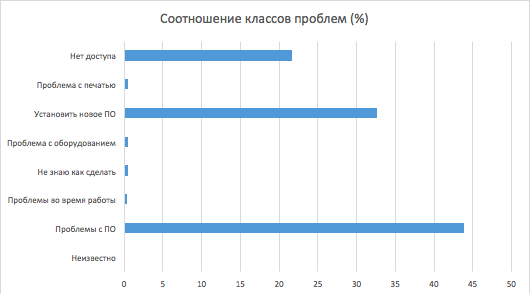
\includegraphics [scale=0.7] {EngineerTasks}
  \label{img:EngineerTasks}  
\end{figure}


\end{frame}


\begin{frame}
\frametitle{Проблемы автоматизации}
\begin{enumerate}
 \item Неоднозначные запросы (примеры);
	\begin{enumerate}
 		\item The installation of Winrar that I got this afternoon did go wrong. During installation nothing else was running. When I tried to start Winrar I got the fault message that is attached here;
 		\item Before i went to vacation i got LOT234, please check if it installed.
	\end{enumerate}
 \item Грамматические ошибки (примеры);
  \begin{enumerate}
 		\item The installation of Winrar that I got this afternoon did go wrong. During installation nothing else was running. When I tried to start Winrar I got the fault message that is attached here.
	\end{enumerate}
	
  \item Запросы на естественном языке.
\end{enumerate}
\end{frame}


\begin{frame}
\frametitle{Имитационная модель процессов обработки инцидентов на базе СМО}
\begin{figure} [h] 
  \center
  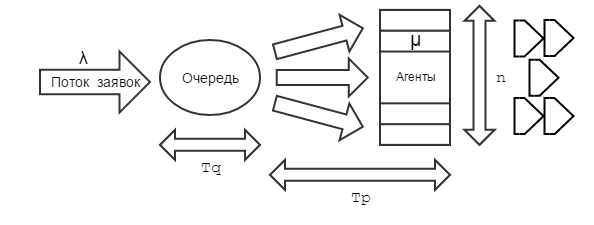
\includegraphics [scale=0.5] {mass_service}
  \label{img:mass_service}  
\end{figure}

\end{frame}

\begin{frame}
\frametitle{Характеристики модели}
\begin{enumerate}
 \item $\lambda$ --- интенсивность входящего потока (заявок в час);
    \item $\alpha$ --- доля заявок, для которых время в очереди превышает $max(T_q)$;       
    \item $\mu$ --- величина, обратная среднему времени нахождения заявки у агента;
	\item  $n$ --- число агентов;
	\item $T_q$ --- время нахождение заявки в очереди в минутах;
	\item SLA=1-$\alpha$ --- уровень обслуживания, доля заявок, для которых время в очереди не превышает $max(T_q)$. 
	\item $T_p$ --- время удовлетворения заявки (час);
 	

\end{enumerate}
\end{frame}

\begin{frame}
\frametitle{Характеристики модели}
\begin{enumerate}
 \item $\alpha_n$ --- количество заявок;
 \item	$T_{qp}=T_q+T_p$ --- время прохождения заявки через систему (час);
 \item	$S(\mu)= \frac{R_p}{\mu} $ --- средняя стоимость выполнения одной заявки;
 \item $R_p$ --- средняя стоимость часа работы специалиста (выводится далее);
 \item \textbf{Данные для моделирования:} $T_{qp}=47,9ч$ при $n=6$; $SLA=0,82$; $\alpha=0,18$;  $\alpha_n=2920$. 
\end{enumerate}
\end{frame}





%
%					CHAPTER 2
%исследования выполнялись для усовершенстования, расширить -публикации
\section[Глава 2]{Глава 2. Модель интеллектуальной системы принятия решений}
\begin{frame}
\frametitle{Созданные модели}
\begin{figure} [h] 
  \center 
  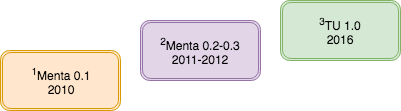
\includegraphics [scale=0.6] {ModelEvolution}
  \caption{Созданные модели} 
  \label{img:ModelEvolution} 
\end{figure}
\begin{minipage}{11cm}
\footnotesize 
\begin{enumerate}
	\item Таланов, М. "Automating programming via concept mining, probabilistic reasoning over semantic knowledge base of SE domain";
	\item Тощев, А, Таланов,  М. "Document Thinking model and machine understanding in automated user request processing";
	\item Тощев, А. "Thinking lifecycle as an implementation of machine understanding in software maintenance domain".
\end{enumerate}
\end{minipage}
\end{frame}


\begin{frame}
\frametitle{Модель $T^3$ по модели Марвина Мински}
\begin{figure} [h] 
  \center
  \includegraphics [scale=0.6] {CSW_EX}
  \caption{Критик~--Селектор~--Путь мышления в разрезе ресурсов} 
  \label{img:csw_ex} 
\end{figure}
\end{frame}

% модель дальше
\begin{frame}
\frametitle{Формальное описание системы}
\begin{figure} [h] 
  \center
  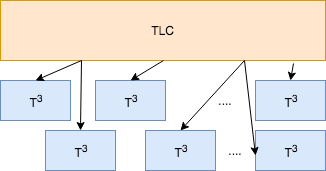
\includegraphics [scale=0.6] {SystemOverview.png}
  \caption{Формальное описание системы. TLC~--- Thinking lifecycle. $T^3$~--- модуль, построенный по принципу $T^3$.} 
  \label{img:SystemOverview.png} 
\end{figure}

\end{frame}

% вместо возвращает - вычисляет вероятность

\begin{frame}
\frametitle{Принцип функционирования}
\begin{enumerate}
	\item Процессы:
\begin{enumerate}
	\item Слабосвязанные;
	\item Короткоживущие.
\end{enumerate}
\item Вероятностные состояния;
\item Примеры процессов;
\begin{enumerate}
	\item Лексико-семантический анализ;
	\item Классификация.
\end{enumerate}
\end{enumerate}
\end{frame}





%
%					CHAPTER 3
%
% перехожу к описанию третий главы
\section[Глава 3]{Глава 3. Реализация модель TU 1.0}



\begin{frame}
\frametitle{Диаграмма действий системы TU}
\begin{figure} [h] 
  \center
  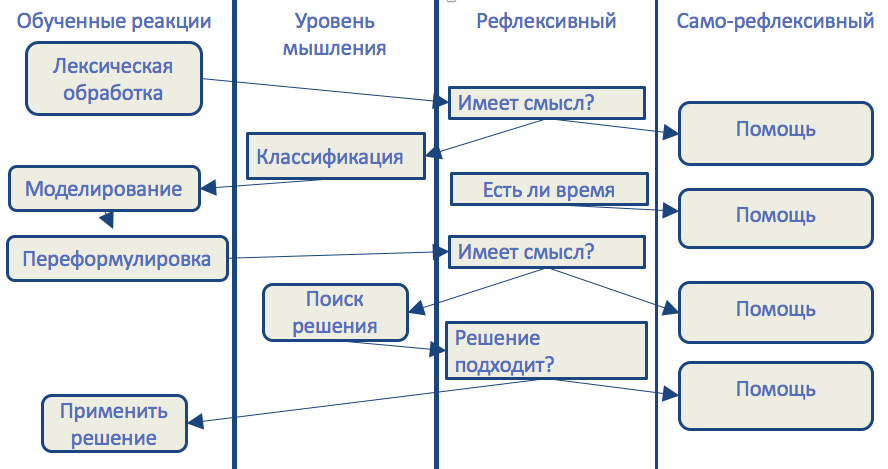
\includegraphics [scale=0.35] {ShortLefecycle}
  \label{img:ShortLefecycle}  
\end{figure}
\end{frame}


\begin{frame}
\frametitle{Пример обработки запроса "Please install Firefox"}
\begin{enumerate}
	\item Возникает инцидент, связанный с запросом от пользователя;
	\item TLC выставляет цель ProcessIncident. К каждой цели привязан набор критиков (каждый критик действует как отдельная вероятностная машина);
	\item PreliminarySplitter обрабатывает входящий запрос с помощью обработчика Link Grammar, который преобразует данное предложение в граф. Этот граф отражает результат лексического и синтаксического разбора.
\end{enumerate}
\end{frame}



\begin{frame}
\frametitle{Результат лексического разбора (Link Grammar)}
\begin{table}
	
\small
\begin{tabular} {|p{5cm}|p{5cm}|}

\hline
 
\_advmod(install, please)
\_obj(install, Firefox)
pos(install, verb)
inflection-TAG(install, .v)
tense(install, imperative)
pos(please, adv)
 & 
inflection-TAG(please, .e)
pos(., punctuation)
noun\_number(Firefox, singular
definite\-FLAG(Firefox, T)
pos(Firefox, noun) 
    \\
   \hline
\end{tabular}
\end{table}

\begin{figure} [h] 
  \center
  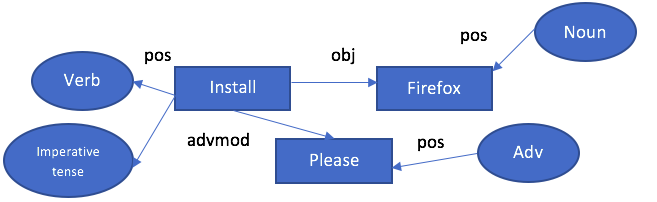
\includegraphics [scale=0.45] {LexicalGraph1}
  \label{img:LexicalGraph1}  
\end{figure}
\end{frame}

%Модуль содержит ограничение на количество предложений и количество слов. Длина предложения не более 1024 символов.
%Модуль содержит ограничение на количество предложений и количество слов. Длина предложения не более 1024 символов.
%1.	Граф, изображенный на Рисунке 1, подвергается разбору и преобразуется во фразы, которые группируются в предложения. В исходном примере нет идиом, но если такие встречаются, то они также будут составлять одну фразу. Отношения, начинающиеся с подчеркивания, – это связи между нодами графа, остальное – это описания конкретного слова. Ссылка может идти также не на лист, а на нод дерева, для этого алгоритм построен рекурсивно. У каждого нода графа есть именованные ссылки, в нашем случае мы берем только ссылки вида: "_subj" (подлежащие); "_obj" (дополнение); "_iobj" (косвенное дополнение); "_advmod" (наречие); "of" (принадлежность). На выходе мы получаем граф, перефразированный в рамках объектов приложения, – AnnotatedPhrase. Кроме того, будут отфильтрованы лишнее связи, также копируются свойства pos (часть речи), tense (время);


\begin{frame}
\frametitle{Вид графа запроса после обработки}
\begin{figure} [h] 
  \center
  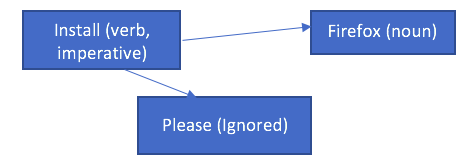
\includegraphics [scale=0.5] {LexicalGraph2}
  \label{img:LexicalGraph2}  
\end{figure}
Используются только "\_subj" (подлежащие); "\_obj" (дополнение); "\_iobj" (косвенное дополнение); "\_advmod" (наречие); "of" (принадлежность).
\end{frame}


%1.	Результат передается в LinkParser, который ищет соответствие между словами, выявленными в разборе, и базой знаний. Например, install уже есть в базе и он получит ссылку на концепцию в базе. Каждая концепция в базе поддерживает свойства generalization, specialization. Рассмотрим концепцию install;

\begin{frame}
\frametitle{Связь с концепциями из базы знаний}
Построенный граф передается в модуль LinkParser, который устанавливает соответствие между словами, выявленными на этапе разбора запроса, и базой знаний. Например, если термин "install" уже есть в БЗ, то он получит ссылку на соответствующую концепцию в БЗ. Каждая концепция в базе поддерживает свойства generalization, specialization. Рассмотрим концепцию install.
\begin{figure} [h] 
  \center
  
\includegraphics [scale=0.5] {Generalisation1}
  \label{img:Generalisation1}  
\end{figure}
\end{frame}


%1.	TLC Выставляет цель ClassifyIncident, и запускаются машины классификации, например, машина DirectInstrutctionAnalyser. Первым этапом он смотрит, есть ли действие в запросе. Во фразе оно есть, значит, итоговая вероятность не уменьшается (по умолчанию итоговая вероятность 1), иначе взвешенный результат будет меньше, так как данный критик нацелен только на действие и объект, над которым нужно его совершить. Далее ищется объект в количестве 1 и прилинкованная к действию. Если они найдены, то итоговая вероятность не уменьшается. 
%Для достижения подсчета итоговой вероятности критик содержит в себе набор правил, который обрабатывается логической машиной PLN. На вход подается граф, изображенный на Рисунке 2, на выходе получается вероятность соответствия графа правилам. Например, правила вида «Граф содержит концепцию подлежащего» или «У нода графа действия есть связь с нодом типа дополнение». В интерпретаторе правил есть поддержка прямой логики ”forward chaining”: конъюнкция, дизъюнкция, отрицания, равно, меньше;


%1.	TLC выставляет цель SearchSolution; так как решения еще нет в базе, то начинается поиск решения путем сравнения графа исходной проблемы и хранящегося в базе знаний решений. Во время поиска идет сравнение изоморфизма графов исходной проблемы и решения, хранящегося в базе знаний. В результате подсчитывается коэффициент удаленности графов – d. Если d = 0, то графы идентичны. Во время подсчета учитывается ссылка на обобщенные концепции. Например, если есть две концепции Winrar и Archive, обе ссылаются на базовую концепцию Software, то соответствие данной вершины будет 0.5, в зависимости от отдаление базовой концепции соответствие будет падать: 0,75; 0,865 и т.д.; 



\begin{frame}
\frametitle{Процесс поиска решения}
%Во время поиска идет сравнение изоморфизма графов исходной проблемы и решения, хранящегося в базе знаний. В результате подсчитывается коэффициент удаленности графов – d. Если d = 0, то графы идентичны. Во время подсчета учитывается ссылка на обобщенные концепции. Например, если есть две концепции Winrar и Archive, обе ссылаются на базовую концепцию Software, то соответствие данной вершины будет 0.5, в зависимости от отдаление базовой концепции соответствие будет падать: 0,75; 0,865 и т.д.; 
Во время поиска идет сравнение изоморфизма графов исходной проблемы и решения, хранящегося в базе знаний.
\begin{figure} [h] 
  \center
  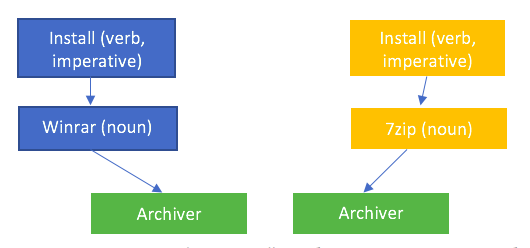
\includegraphics [scale=0.5] {SolutionSearch1}
  \label{img:SolutionSearch1}  
\end{figure}
\end{frame}

\begin{frame}
\frametitle{Пример обработки сложного запроса}
The installation of Winrar that I got this afternoon did go wrong. During installation nothing else was running. When I tried to start Winrar I got the fault message that is attached here.
\begin{figure} [h] 
  \center
  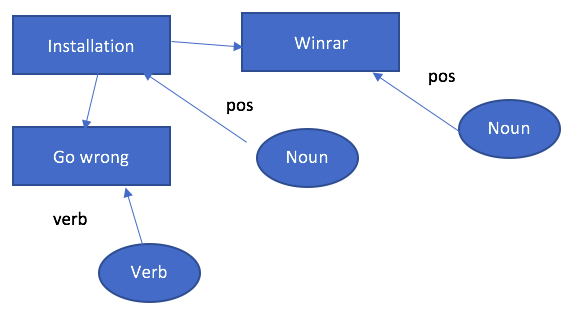
\includegraphics [scale=0.5] {Request2}
  \label{img:Request2}  
\end{figure}
\end{frame}


\begin{frame}
\frametitle{Пример обработки запроса с желаемым состоянием}
I have Office 2010 installed, but I need office 2016.
\begin{figure} [h] 
  \center
  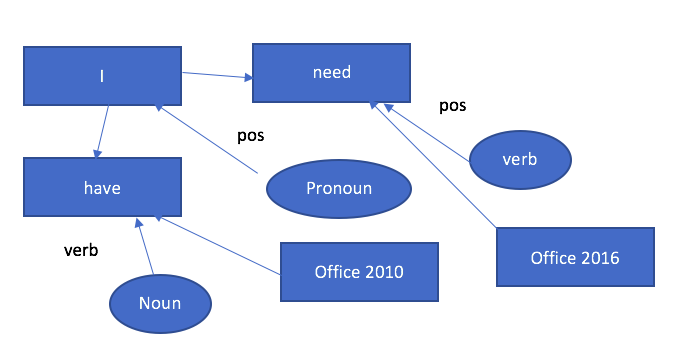
\includegraphics [scale=0.5] {Request3}
  \label{img:Request3}  
\end{figure}
\end{frame}


\begin{frame}
\frametitle{Полная диаграмма действий}

\begin{figure} [h] 
  \centering
  \begin{minipage}{50pt}
  	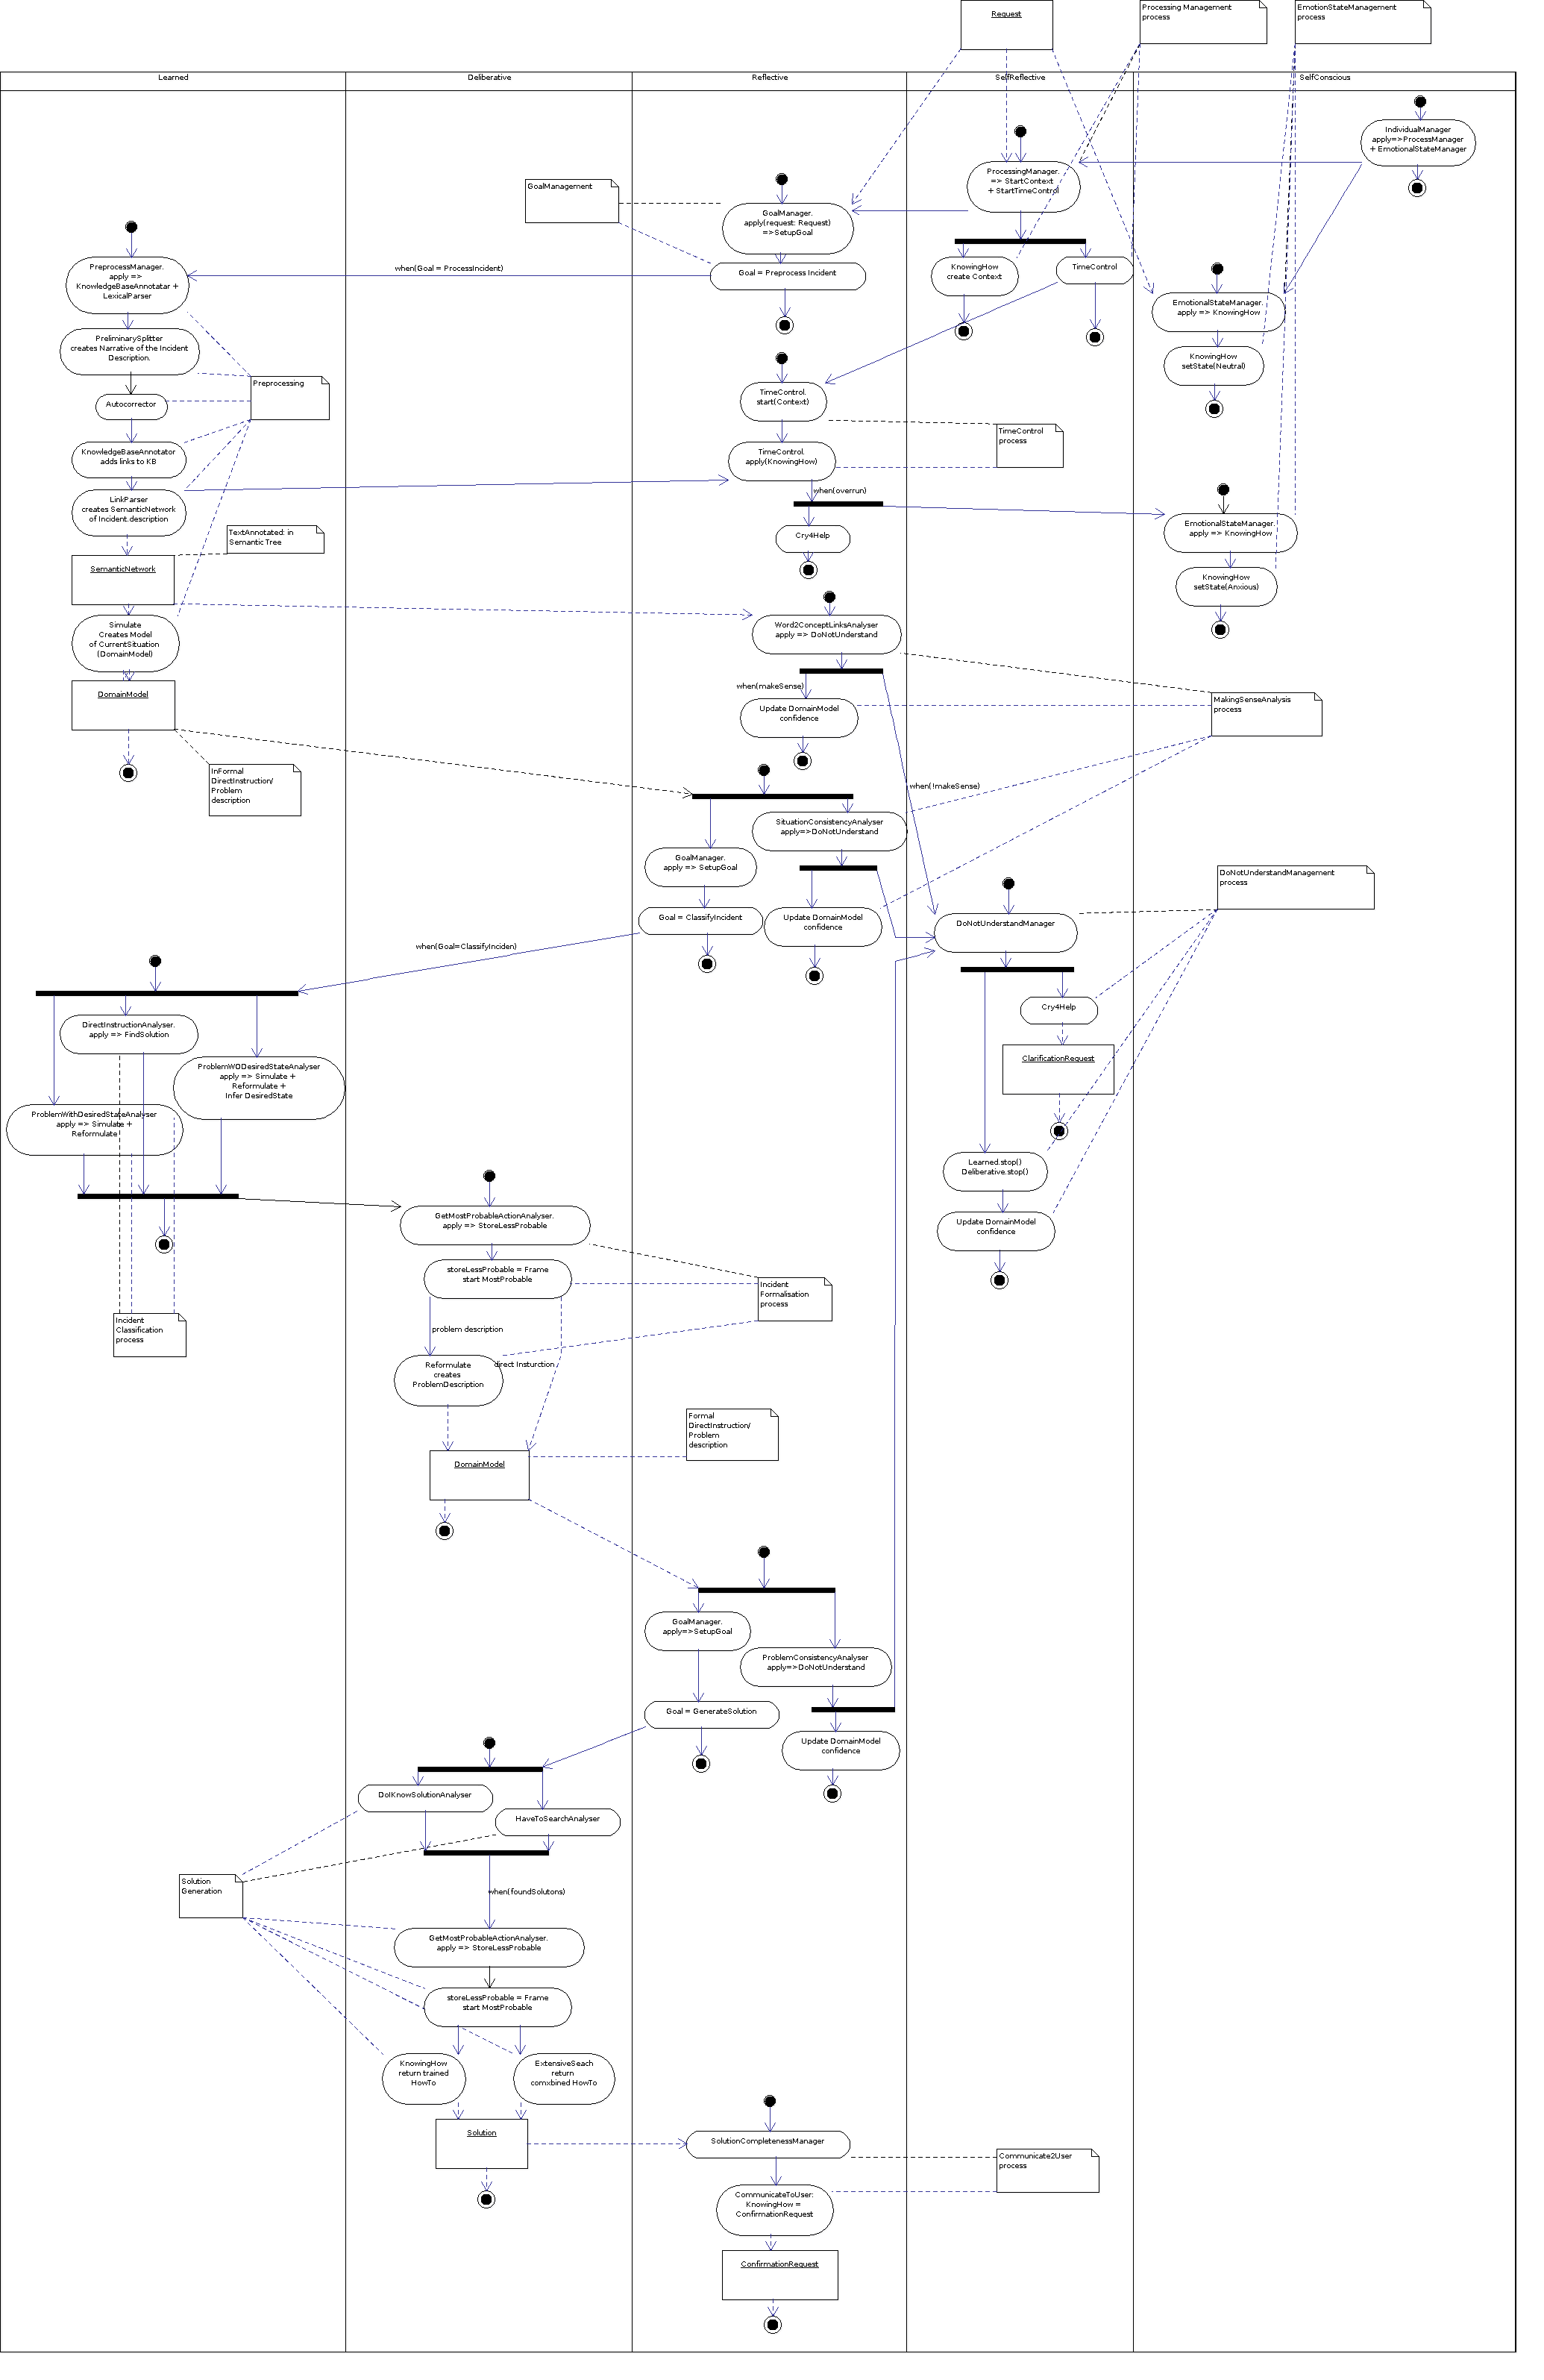
\includegraphics [scale=0.05] {LifecycleActivity}
  \end{minipage}
  \hfill
  \begin{minipage}{150pt}
  	 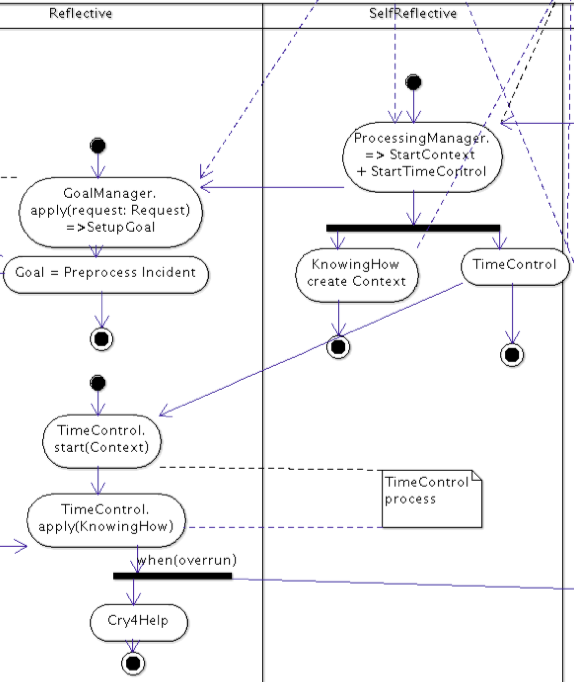
\includegraphics [scale=0.3] {LifecycleShortcut}
  \end{minipage}
  \label{img:LifecycleActivity}  
\end{figure}


\end{frame}

\begin{frame}
\frametitle{Ограничения использования системы}
\begin{enumerate}
	\item Имеется ограничение на длину запроса~--- не более 1024 символов;
	\item Система не может обработать логически противоречивые запросы;
	\item Используются только 5 лексических связей;
	\item Поддерживается только английский язык;
	\item Каждый критик поддерживает не более 8 логических правил.

\end{enumerate}
\end{frame}



\begin{frame}
\frametitle{Особенности системы}
\begin{enumerate}
	\item Представление большинства объектов в Базе Знаний;
	\item Расширяемость;
	\item Масштабируемость за счет Scala Akka;
	\item Концепция ShortTermMemory и LongTermMemory;
	\item Самоконтроль системой своего состояния.
\end{enumerate}
\end{frame}


%
%					CHAPTER 4
%
\section[Глава 4]{Глава 4. Экспериментальные исследования эффективности работы модели TU}



\begin{frame}
\frametitle{Результаты работы}
\begin{table}
	
\small
\begin{tabular} {|p{8cm}|p{1cm}|p{1cm}|}

\hline
%время в милисекундах
\textbf{Запрос} & TSS1 (ms) & TU (ms) \\
\hline
  Tense is kind of concept & 15000 & 385 \\
  
  \hline
  Please install Firefox  & 9000 & 859 \\
  \hline
  Browser is an object   & 20000 & 400 \\
  \hline
  Firefox is a browser   & 5000 & 659  \\
  \hline
  Install is an action    & 8000 & 486 \\
  \hline
  User miss Internet Explorer 8     & 10000 & 10589 \\
  \hline
  User needs document portal update    & 15000 & 16543 \\
  \hline
  Add new alias Host name on host that alias is wanted to: hrportal.lalala.biz IP adress on host that alias is wanted to: 322.223.333.22 Wanted Alias:    webadviser.lalala.net    & 10000 & 18432  \\ 
  \hline
  PP2C - Cisco IP communicator. Please see if you can fix the problem with the <...> & 13000 & 12343 \\ 
   \hline
   \end{tabular}
\end{table}
\end{frame}

\begin{frame}
\frametitle{Результаты работы}
\begin{table}
	
\small
\begin{tabular} {|p{8cm}|p{2cm}|}

\hline
\textbf{Категория} & \textbf{Описание} \\
\hline
 Проблема с ПО    & 64\% \\
 \hline Проблемы во время работы  &  10\% \\
  \hline Как сделать & 10\% \\
   \hline
Проблема с оборудованием  & 0\% \\
 \hline
Установить новое ПО       & 100\% \\
 \hline Проблема с печатью        & 80\% \\
  \hline Нет доступа               & 100\% \\
  \hline
   \end{tabular}
\end{table}

\end{frame}

\begin{frame}
\frametitle{Результаты моделирования}
\begin{enumerate}
 \item \textbf{Результаты моделирования:} $T_{qp}=47,9ч$ при $n=6$; $SLA=0,82$; $\alpha=0,18$;  $\alpha_n=2920$;
 \item \textbf{Результаты моделирования с помощью TU:} $T_{qp}=32,9ч$ при $n=8$; $SLA=0,96$; $\alpha=0,04$;  $\alpha_n=2920$.
\end{enumerate}
\end{frame}


%
%					Conclusions
%
\section[Заключение]{Заключение}



%%%%%%%%%%%%%%%%%%%%%%%%%%%%%%
\begin{frame}
\frametitle{Основные результаты работы}
\begin{itemize}
   \item Создана модель проблемно-ориентированной системы управления знаниями в области обслуживания информационной инфраструктуры предприятия на основе обобщения модели мышления;
  \item Представлены новая модель данных для модели мышления и оригинальный способ их хранения, более эффективный по сравнению с классическими базами данных, использующими реляционный подход;
  \item  Выполнено оригинальное исследование моделей мышления в области обслуживания информационной инфраструктуры предприятия;
  
\end{itemize}
\end{frame}


\begin{frame}
\frametitle{Основные результаты работы}
\begin{itemize}
   \item На основе модели, разработанной в диссертации, созданы архитектура системы и ее прототип; 
   \item Представлена визуализация структуры области удаленной поддержки инфраструктуры.
\end{itemize}
\end{frame}


\begin{frame}
\frametitle{Свидетельство о регистрации ПО}
\begin{figure} [h] 
  \center
  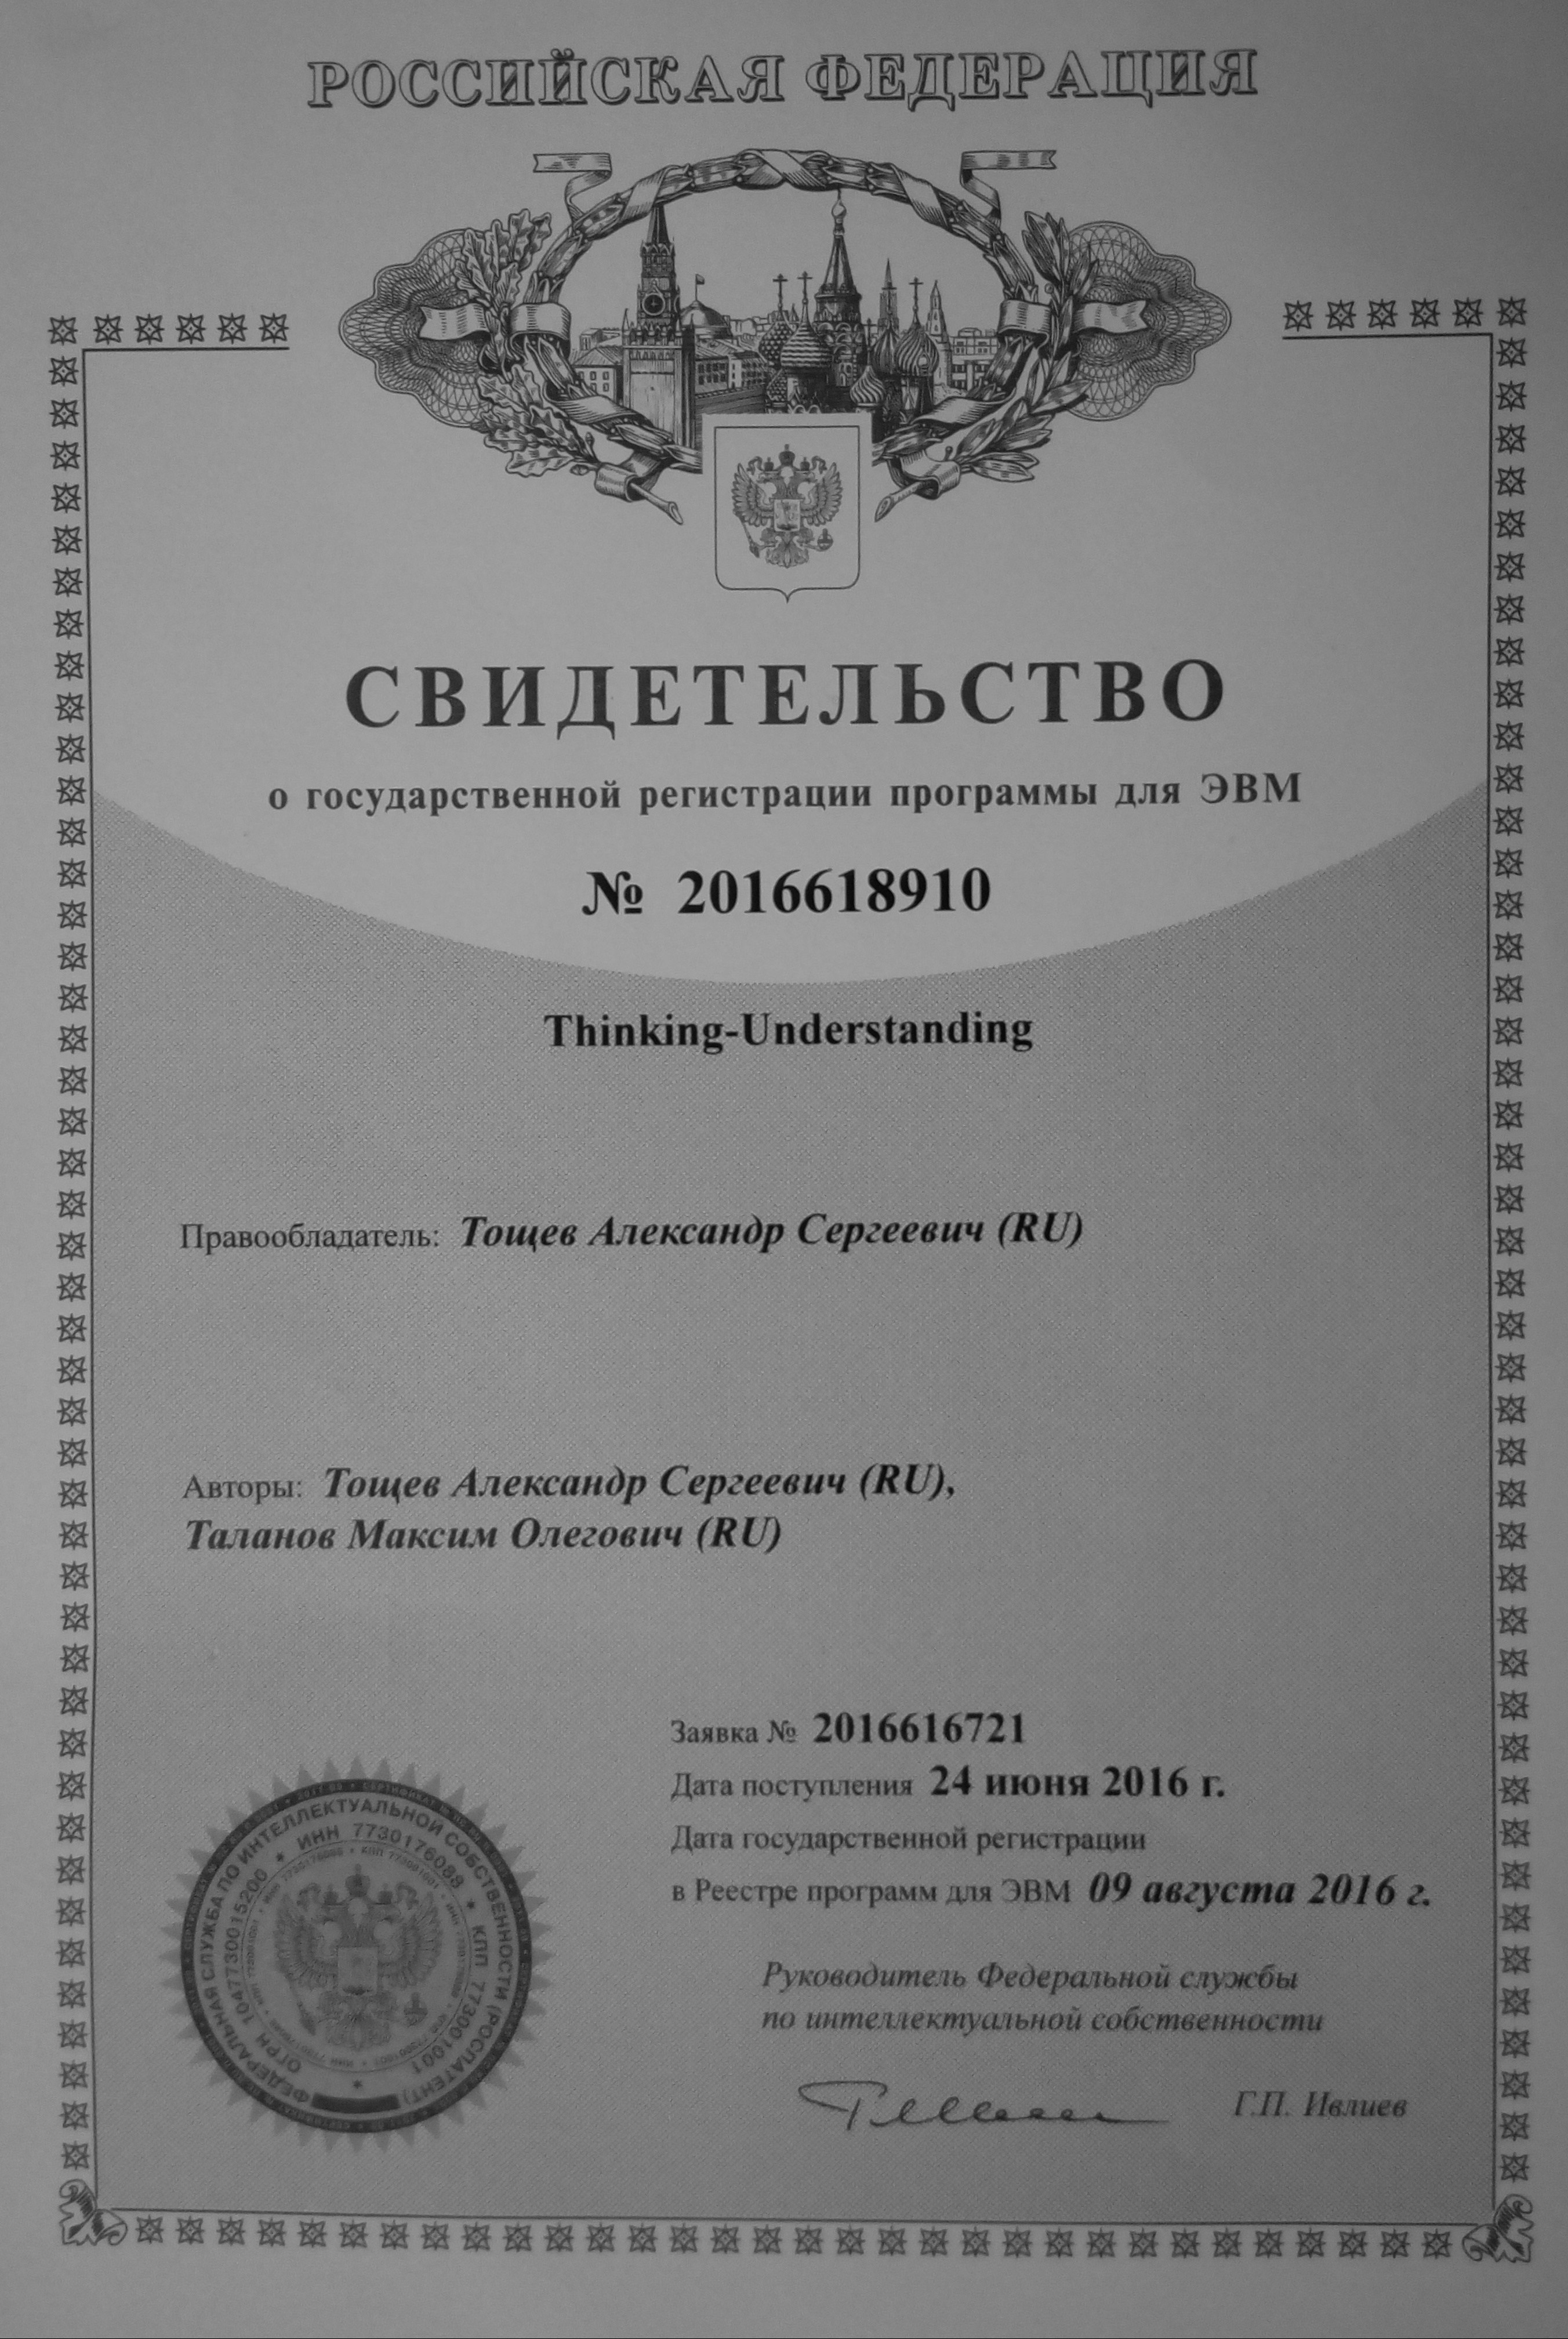
\includegraphics [scale=0.05] {RegistrationStatement}
  \label{img:RegistrationStatement}  
\end{figure}

\end{frame}


\begin{frame}
\frametitle{Акт о внедрении ПО}
\begin{figure} [h] 
  \center
  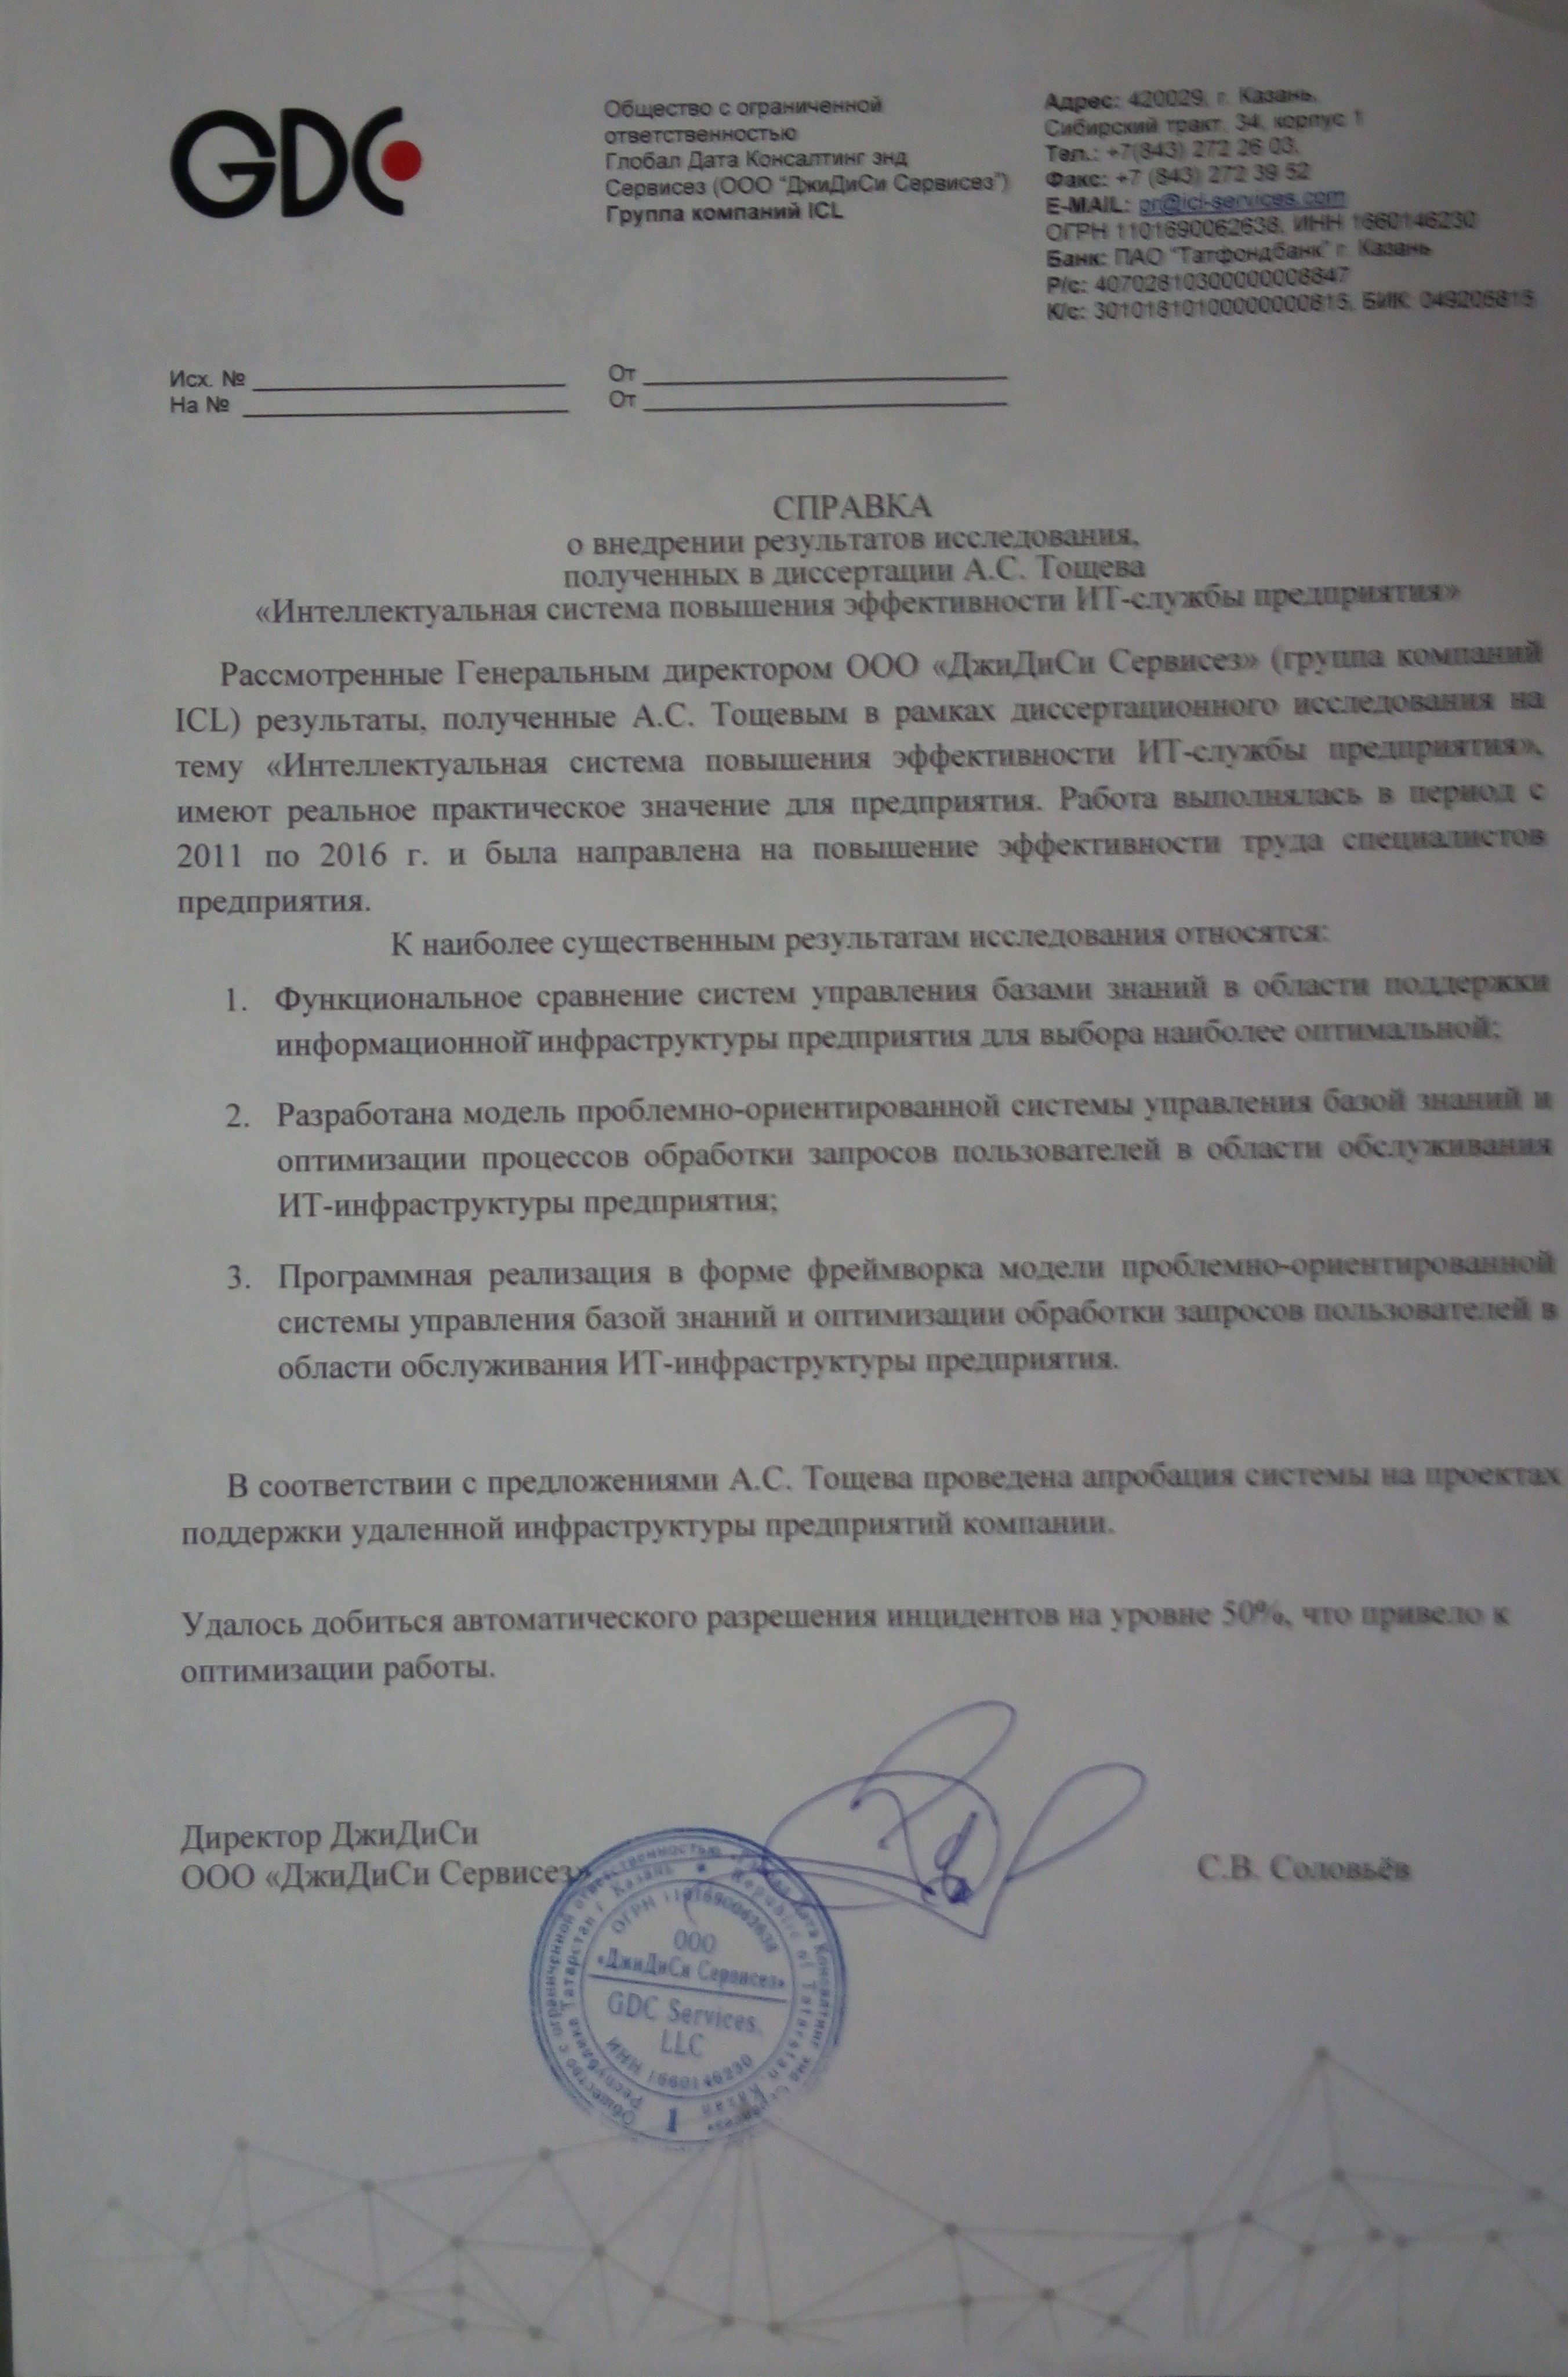
\includegraphics [scale=0.05] {ActVnedr} 
  \label{img:ActVnedr}  
\end{figure}



\end{frame}


\begin{frame}
\begin{center}
Спасибо за внимание!
\end{center}
\end{frame}

%%%%%%%%%%%%%%%%%%%%%%%%%%%%%%
%additional

\begin{frame}
\frametitle{6 уровней мышления}
\begin{enumerate}
	\item Самосознательный уровень;
	\item Саморефлексивный уровень;
	\item Рефлексивные размышления;
	\item Уровень рассуждений;
	\item Уровень обученных реакций;
	\item Инстинктивный.
\end{enumerate}
\end{frame}

\begin{frame}
\frametitle{Обработка запроса}
\begin{figure} [h] 
	\center
	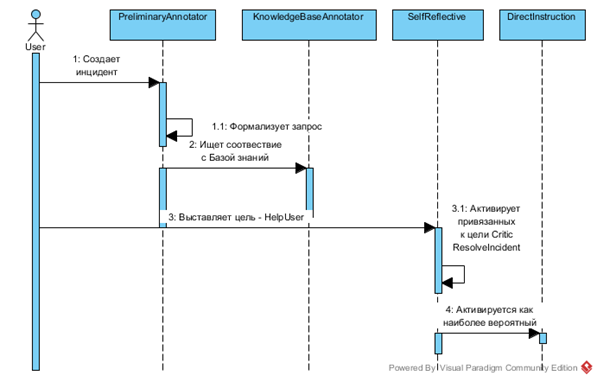
\includegraphics [scale=0.7] {RequestProcesssing}
	\label{img:RequestProcesssing}  
\end{figure}
\end{frame}

\begin{frame}
\frametitle{Обработка запроса}
\begin{figure} [h] 
	\center
	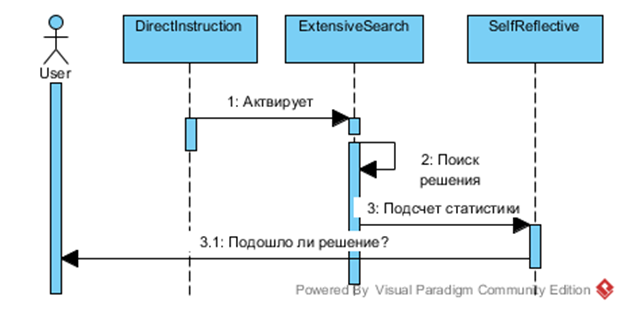
\includegraphics [scale=0.7] {RequestProcesssing2}
	\label{img:RequestProcesssing2}  
\end{figure}
\end{frame}


\begin{frame}
\frametitle{Диаграмма состояний объектов}
\begin{figure} [h] 
  \center
  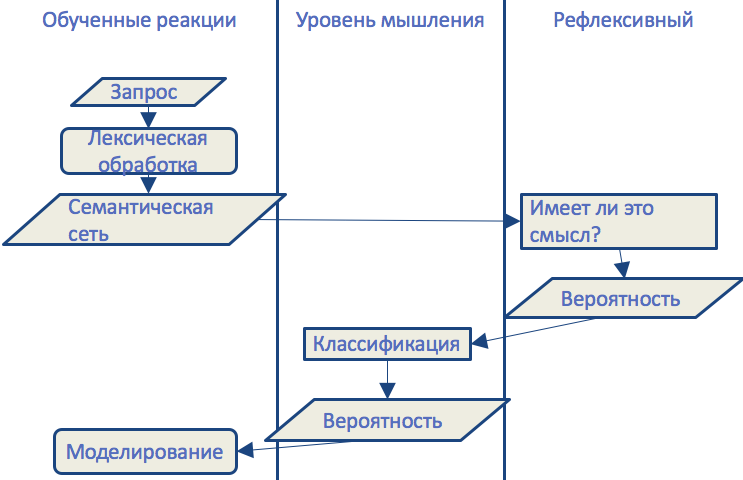
\includegraphics [scale=0.35] {ObjectState}
  \label{img:ObjectState}  
\end{figure}
\end{frame}


\begin{frame}
\frametitle{Специальность}
\begin{enumerate}
    \item Специальность 05.13.11 (технические науки), «Математическое и программное обеспечение вычислительных машин, комплексов и компьютерных сетей».
\end{enumerate}
\end{frame}

\begin{frame}
\frametitle{База знаний}
\begin{enumerate}
	\item Resource;
	\item Semantic Network;
	\item Rule;
	\item KLine;
	\item Neo4j.
\end{enumerate}
\end{frame}




%Структура диссертации
\begin{frame}
\frametitle{Структура диссертации}
\begin{enumerate}
\item \textbf{Введение}
  \item \textbf{Глава 1. Интеллектуальные системы регистрации и анализа проблемных ситуаций, возникающих в ИТ-инфраструктуре предприятия}
  \begin{itemize}
    \item Обзор исследований в области интеллектуальных систем регистрации и анализа проблемных ситуаций;
    \item Сравнительный анализ систем регистрации и устранения проблемных ситуаций;
    \item Сравнительный анализ методов и комплексов обработки текстов на естественном языке;
    \item Выводы по главе 1.
  \end{itemize}
 \end{enumerate}
\end{frame}

\begin{frame}
\frametitle{Структура диссертации}
\begin{enumerate}
  \item \textbf{Глава 2. Модель интеллектуальной системы принятия решений для регистрации и анализа проблемных ситуаций в ИТ-инфраструктуре предприятия}
  \begin{itemize}
    \item Построение модели Menta 0.1 с использованием деревьев принятия решений;
    \item Модель Menta 0.3, построенная с использованием генетических алгоритмов;
    \item Модель TU 1.0, основанная на модели мышления Марвина Мински;
    \item Выводы по главе 2.
  \end{itemize}
\end{enumerate}
\end{frame}

\begin{frame}
\frametitle{Структура диссертации}
\begin{enumerate}
  \item \textbf{Глава 3. Реализация модели TU 1.0 для системы интеллектуальной регистрации и устранения проблемных ситуаций}
  \begin{itemize}
    \item Архитектура системы;
    \item Модель данных TU Knowledge;
    \item Прототип системы;
    \item Выводы по главе 3.
  \end{itemize}
   \item \textbf{Глава 4. Экспериментальные исследования эффективности работы модели TU}
  \begin{itemize}
    \item Экспериментальные данные;
    \item Оценка эффективности;
    \item Результаты экспериментов;
    \item Выводы по главе 4.
  \end{itemize}

\end{enumerate}
\end{frame}

%%%%%%%%%%%%%%%%%%%%%%%%%%%%%%%%%%%%%%%


\end{document} 